\documentclass[titlepage,a4paper,12pt]{report}
\usepackage{amssymb,amsfonts,amsmath}
\usepackage{tikz}
\usetikzlibrary{arrows}
\newcommand\Interval[4]{%
  \begin{tikzpicture}[text height=1ex]%
    \draw[<-] (0,0) -- (1,0);
    \draw[{#3-#4}] (1,0) node[label=below:{#1}] {} -- (2,0) node[label=below:{#2}] {};
    \draw[->] (2,0) -- (3,0);
  \end{tikzpicture}
}
%\usepackage{fullpage}
\usepackage{graphicx}
%\usepackage[cc]{titlepic}
\usepackage{amsthm}
\newtheorem{definition}{Definition}[section]
\newtheorem{example}{Example}[section]
\newtheorem{theorem}{Theorem}[section]
\newtheorem{exercise}{Exercise}[section]
\newtheorem{corollary}{Corollary}[section]
\newtheorem{proposition}{Proposition}[section]
\pdfpagewidth 8.5in
\pdfpageheight 11in
\setlength\topmargin{-0.5in}
\setlength\headheight{0in}
\setlength\headsep{0in}
\setlength\textheight{9.5in}
\setlength\textwidth{7.0in}
\setlength\oddsidemargin{-0.5in}
\setlength\evensidemargin{1.0in}
\setlength\parindent{0.25in}
\setlength\parskip{0.25in}
%\begin{titlepage}
%\usepackage{titlepic}
%\titlepic{
\includegraphics[width=0.2\textwidth]{uz1.png}}
%
%\title{\textbf{HMTH111 Calculus 2}}
%\author{Nhawu. G\\
%		Department of Mathematics\\
%		University of Zimbabwe, ZIM}
%
%\end{titlepage}

\begin{document}
\begin{titlepage}
 
\begin{center}
 
 
% Upper part of the page

\includegraphics[width=0.15\textwidth]{uz1.png}\\[1cm]
 
\textsc{\LARGE University of Zimbabwe}\\[1.5cm]
 
\textsc{\Large HMTH101 CALCULUS 1}\\[0.5cm]
 
 
% Title

{ \huge \bfseries Calculus of Single Variables}\\[0.4cm]
 

 
% Author and supervisor
\begin{minipage}{0.4\textwidth}
\begin{center} \large
\emph{Author:}\\
G. \textsc{Nhawu}
\end{center}
\end{minipage}
\begin{minipage}{0.4\textwidth}
\begin{flushright} \large
\emph{Department:} \\
\textsc{Mathematics}
\end{flushright}
\end{minipage}

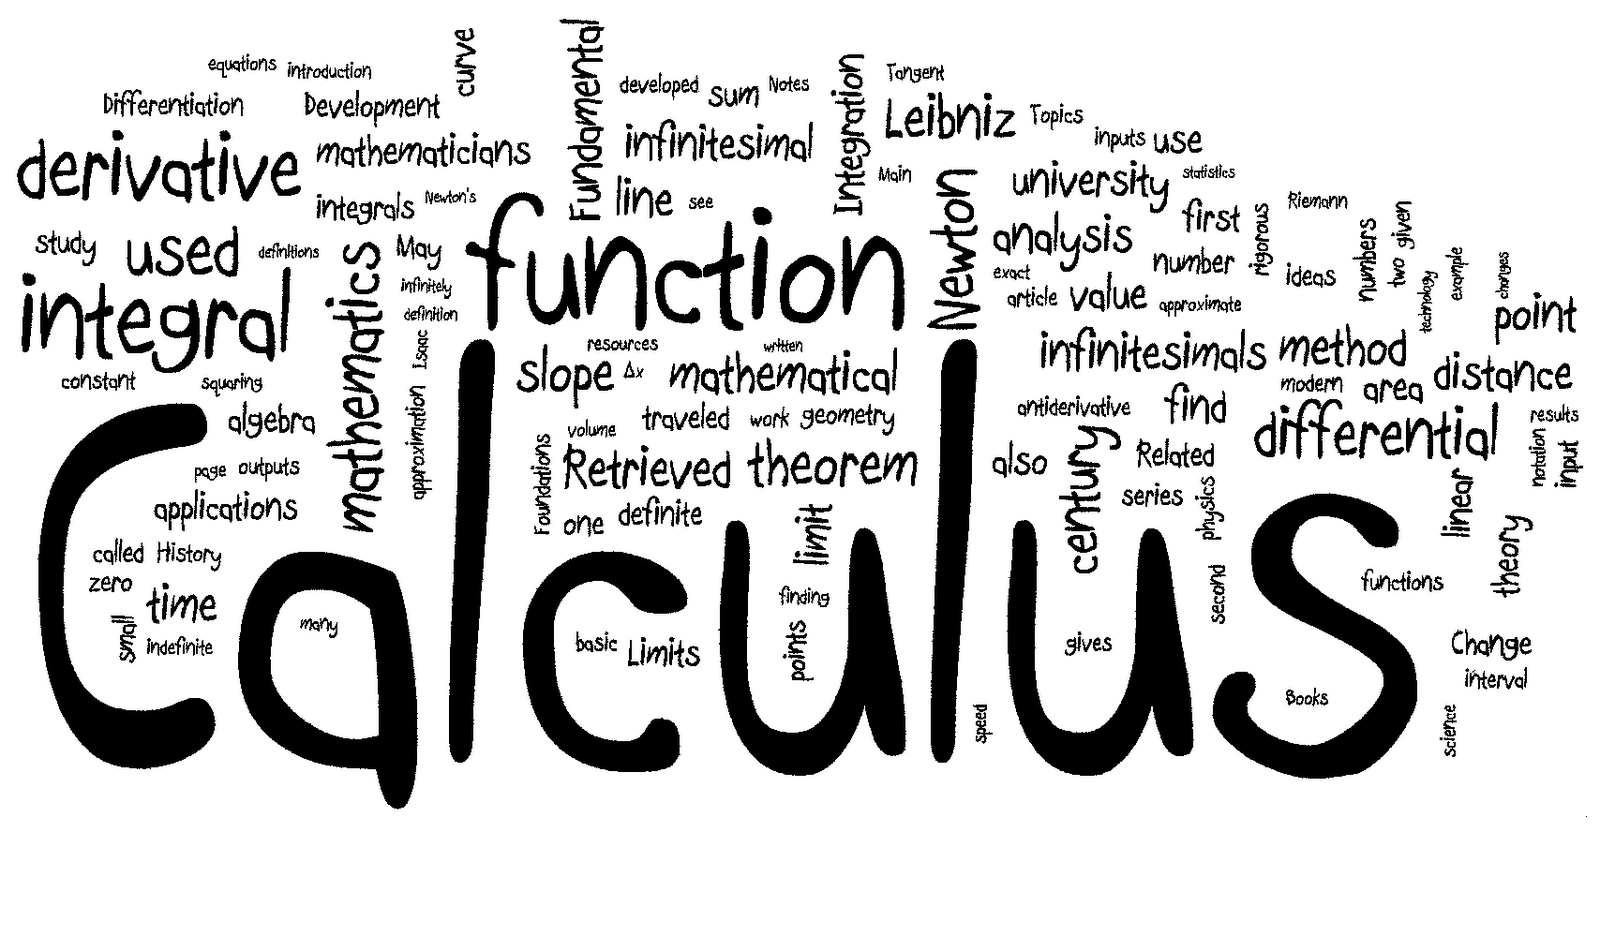
\includegraphics[width=0.98\textwidth]{calculus2.png}\\[1cm]
 \vfill
 
 
% Bottom of the page
{\large \today}
 
\end{center}
 
\end{titlepage}

\tableofcontents
\setcounter{chapter}{5}
\chapter{Applications of the Derivative}
\begin{center}
	\small{\parbox{18cm}{
		\begin{raggedright}
		{\small
		\textit{Gravitation cannot be held responsible for people falling in
love. How on earth can you explain in terms of chemistry
and physics so important a biological phenomenon as first
love? Put your hand on a stove for a minute and it seems
like an hour. Sit with that special girl for an hour and it
seems like a minute. That's relativity.}
 }
 
				\vspace{.5cm}\hfill{---Albert Einstein}
		\end{raggedright}
	}
} 
\end{center}
\section{Approximation by Differentials}
A method for approximating the value of a function near a known value. The method uses the tangent line at a  known value of the function to approximate the function's graph. Let $\Delta x$ and $\Delta y$ represent the changes in $x$ and $y$ for the function and $dx$ and $dy$ represents the changes in $x$ and $y$ for the tangent line.
\begin{center}
 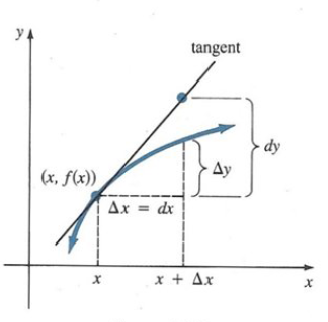
\includegraphics[width=0.4\textwidth]{tan.png}\\[1cm]
  \end{center}
 
\noindent This is also written as 
\begin{equation*}
f(x+\Delta x)=f(x)+\Delta y =f(x)+f'(x)\Delta x.
\end{equation*}

\noindent \textbf{Example:} Approximate $\sqrt{10}$ by differentials.

\noindent \textbf{Solution:} $\sqrt{10}$ is near $\sqrt{9}$, so we will use $f(x)=\sqrt{x}$ with $x=9$ and $\Delta x =10-9=1$. Note that $f'(x)=\dfrac{1}{2\sqrt{x}}$. Therefore
\begin{eqnarray*}
\sqrt{10} &=& f(x+\Delta x)\\
&\approx & f(x)+ f'(x)\Delta x\\
&=& \sqrt{x} +\dfrac{1}{2\sqrt{x}}\Delta x =\sqrt{9} +\dfrac{1}{2\sqrt{9}} (1)\\
&=& \dfrac{19}{6}.
\end{eqnarray*}
\noindent \textbf{Example:} Find an approximate value of $\sqrt[3]{9}$.

\noindent \textbf{Solution:} We set $f(x)=\sqrt[3]{x}$. Suppose to find $f(9)$. Note that $f'(x)=\frac{1}{3}x^{-\frac{2}{3}}$ and hence, $f(8)=2$ and $f'(8)=\frac{1}{12}$, where $x=8$ and $\Delta x =9-8=1$. Therefore, 
\begin{eqnarray*}
\sqrt[3]{9} &=& f(9) \approx 2+\dfrac{1}{12} (1)\\
&=& \dfrac{25}{12}\\
&\approx & 2.0833.
\end{eqnarray*}
 \noindent \textbf{Example:} Find an approximate value for $\tan 46^\circ$.
 
 \noindent \textbf{Solution:} Radial measure $46^\circ =45^\circ +1^\circ$ corresponds to $\dfrac{\pi}{4} +\dfrac{\pi}{180}$ and note that $f(x)=\tan x$, then $f'(x)=\sec ^2 x$ and $f(\frac{\pi}{4})=1, \, f'(\frac{\pi}{4})=2$. Therefore
 \begin{equation*}
 \tan 46^\circ = \tan \left(\dfrac{\pi}{4}+\dfrac{\pi}{180}\right) \approx \tan \frac{\pi}{4} +\sec ^2 \frac{\pi}{4} \left(\dfrac{\pi}{180}\right) = 1+\dfrac{\pi}{90} \approx 1.0349.
 \end{equation*} 
 \section{The Mean Value Theorem}
 Suppose $f(x)$ is continuous on $[a,b]$ and differentiable on $(a,b)$. Then, there exists a $c$ in $(a,b)$ at which the tangent line is parallel to the secant line joining the points $(a,f(a))$ and $(b,f(b))$, i.e., at which $f'(c)=\dfrac{f(b)-f(a)}{b-a}$, 
 
 \noindent \textbf{OR} \\
 
 
\noindent  If $f(x)$ is continuous in $[a,b]$ and differentiable in $(a,b)$, then there exists a point $c$ in $(a,b)$ such that 
 \begin{equation*}
 f'(c)=\dfrac{f(b)-f(a)}{b-a}, \quad a<c<b.
 \end{equation*}
 \begin{center}
 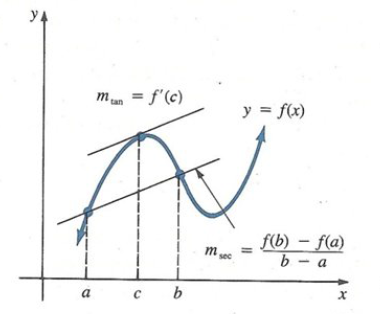
\includegraphics[width=0.4\textwidth]{mean.png}\\[1cm]
  \end{center}
 \noindent The word \textbf{mean} in The Mean Value Theorem refers to the mean (or average) rate of change of $f$ in the interval $[a,b]$.
 
 
\noindent If $f(a)=f(b)=0$, then the theorem says that there exists a $c$ in $(a,b)$ at which $f'(c)=0$. The graphs suggest that there must be at least one point on the graph, that corresponds to a number $c$ in $(a,b)$, at which the tangent is horizontal. This special case of the Mean Value Theorem is called \textbf{Rolle's Theorem} \footnote{Michel Rolle, a French mathematician (1652-1719)}. 
\begin{center}
 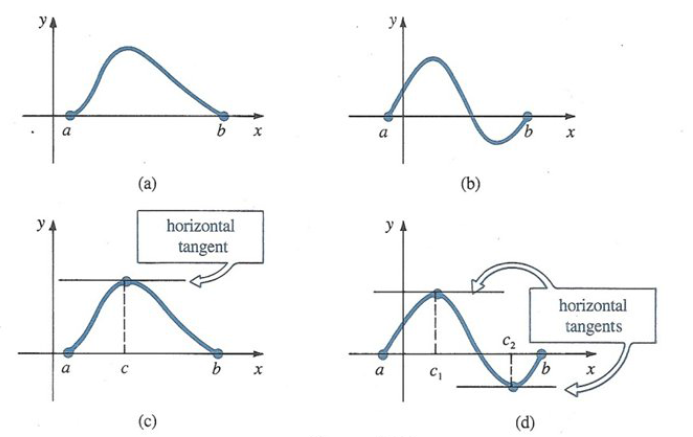
\includegraphics[width=0.6\textwidth]{rolle.png}\\[1cm]
  \end{center}
\noindent \textbf{Example:} Consider $f(x)=\sqrt{x-1}$ on $[2,5]$, $f(x)$ is continuous when $x-1\geq 0$, i.e., $x\geq 1$. In particular, $f(x)$ is continuous on $[2,5]$ and $f'(x)=\dfrac{1}{2\sqrt{x-1}}$, so differentiable when $x>1$. In particular, $f(x)$ is differentiable on $(2,5)$. 
\begin{equation*}
\dfrac{f(b)-f(a)}{b-a} =\dfrac{f(5)-f(2)}{5-2} =\dfrac{\sqrt{5-1}-\sqrt{2-1}}{3}=\dfrac{1}{3}.
\end{equation*} 
The Mean Value Theorem asserts that, for some $c$ in $(2,5), \, f'(c)=\dfrac{1}{3}$. Let us find it.
\begin{eqnarray*}
f'(x) &=&\dfrac{1}{3}\\
\dfrac{1}{2\sqrt{x-1}} &=&\dfrac{1}{3}\\
2\sqrt{x-1} &=& 3\\
4(x-1) &=& 9\\
x-1 &=&\dfrac{9}{4}\\
x &=& \dfrac{13}{4}.
\end{eqnarray*}
Notice that $\dfrac{13}{4}$ is in $(2,5)$, so we may take $c=\dfrac{13}{4}$.

\noindent \textbf{Example:} Show that if $f(x)=\tan x$ on the interval $0\leq x\leq k$ where $k<\dfrac{\pi}{2}$, then $\tan k \geq k$.

\noindent \textbf{Solution:} By the Mean Value Theorem
\begin{equation*}
\dfrac{\tan k -\tan 0}{k-0} =\sec ^2 c,
\end{equation*}
 for some $c\in (0,k)$. But $\sec ^2 c \geq 1$ and $\tan 0 =0$. So 
 \begin{equation*}
 \dfrac{\tan k}{k} \geq 1 \Longrightarrow \tan k \geq k.
 \end{equation*}
 
 \noindent \textbf{Example:} Use The Mean Value Theorem to show that $|\cos a -\cos b|\leq |a-b|$.
 
 \noindent \textbf{Solution:} The function $\cos x$ is continuous and differentiable for all $x$. By the Mean Value Theorem
 \begin{eqnarray*}
 (\cos x)' &=& \dfrac{\cos a -\cos b}{a-b}\\
 |(\cos x)'| &=& \left|\dfrac{\cos a -\cos b}{a-b} \right|,
 \end{eqnarray*}
 but $(\cos x)'=-\sin x$ and $|(\cos x)'|\leq 1$, therefore
 \begin{equation*}
 \dfrac{|\cos a -\cos b|}{|a-b|}\leq 1 \Longrightarrow |\cos a -\cos b|\leq |a-b|.
 \end{equation*}
 
 \noindent \textbf{Example:} Prove that $\dfrac{b-a}{1+b^2}<\tan ^{-1} b -\tan ^{-1} a < \dfrac{b-a}{1+a^2}$ for $a<b$.
 
 \noindent \textbf{Solution:} Let $f(x)=\tan ^{-1} x $. Since $f'(x)=\dfrac{1}{1+x^2}, \,f'(c)=\dfrac{1}{1+c^2} $. By the Mean Value Theorem
 \begin{equation*}
 \dfrac{f(b)-f(a)}{b-a}=\dfrac{\tan ^{-1} b-\tan ^{-1} a}{b-a} =\dfrac{1}{1+c^2}, \quad a<c<b.
 \end{equation*}
 Then, from $a<c<b$, we have 
 \begin{eqnarray*}
 a^2<c^2<b^2 &\Longrightarrow& 1+a^2<1+c^2<1+b^2\\
 \dfrac{1}{1+a^2}>\dfrac{1}{1+c^2}>\dfrac{1}{1+b^2} &\Longrightarrow &  \dfrac{1}{1+b^2}<\dfrac{1}{1+c^2}<\dfrac{1}{1+a^2}\\
 \dfrac{1}{1+b^2}<\dfrac{\tan ^{-1} b -\tan ^{-1} a}{b-a} <\dfrac{1}{1+a^2} &\Longrightarrow & \dfrac{b-a}{1+b^2}<\tan ^{-1} b -\tan ^{-1} a < \dfrac{b-a}{1+a^2}.
 \end{eqnarray*}
 
 \noindent \textbf{Example:} Use the Mean Value Theorem, to prove that if $0<a<b$, then $1-\dfrac{a}{b}<\ln \left(\dfrac{b}{a}\right)<\dfrac{b}{a}-1$. Hence show that $\dfrac{1}{6}<\ln 1.2 < \dfrac{1}{5}$.
 
 \noindent \textbf{Solution:} Let $f(x)=\ln x$ and $f'(x)=\dfrac{1}{x}$. By the Mean Value Theorem, there exists $c\in (a,b)$ such that 
 \begin{equation*}
f'(c)=\dfrac{1}{c}=\dfrac{\ln b -\ln a}{b-a}. 
 \end{equation*}
 Then, from $a<c<b$ we have
 \begin{eqnarray*}
 a<c<b  &\Longrightarrow & \dfrac{1}{b}< \dfrac{1}{c} <\dfrac{1}{a} \\
 \dfrac{1}{b} <\dfrac{\ln b -\ln a}{b-a} <\dfrac{1}{a} &\Longrightarrow & \dfrac{b-a}{b}<\ln b -\ln a < \dfrac{b-a}{a}\\
 &\Longrightarrow & 1-\dfrac{a}{b}<\ln \left(\dfrac{b}{a}\right)<\dfrac{b}{a}-1.
 \end{eqnarray*}
 
\noindent Now, $\ln (1.2)=\ln \left(\dfrac{12}{10}\right)=\ln \left(\dfrac{6}{5} \right)$. Therefore $a=5$ and $b=6$. Substituting in \\$1-\dfrac{a}{b}<\ln \left(\dfrac{b}{a}\right)<\dfrac{b}{a}-1$, we have 
\begin{equation*}
1-\dfrac{5}{6}<\ln \left(\dfrac{6}{5}\right)<\dfrac{6}{5}-1 \Longrightarrow \dfrac{1}{6}<\ln 1.2 < \dfrac{1}{5}.
\end{equation*}
\section{Some Corollaries of The Mean Value Theorem}
\begin{corollary}
If $f'(x)=0$ at all points of the interval $(a,b)$, then $f(x)$ must be a constant in the interval.
\end{corollary}
\begin{proof}
Let $x_1<x_2$ be any two different points in $(a,b)$. By the Mean Value Theorem for\\
 $x_1<x<x_2$, 
\begin{equation*}
\dfrac{f(x_2)-f(x_1)}{x_2-x_1} =f'(x)=0.
\end{equation*} 
Thus $f(x_1)=f(x_2)$. Since $x_1$ and $x_2$ are arbitrarily chosen, the function $f(x)$ has the same value at all points in the interval. Thus, $f(x)$ is constant.
\end{proof}
\begin{corollary}
If $f'(x)>0$ at all points of the interval $(a,b)$, then $f(x)$ is strictly increasing.
\end{corollary}
\begin{proof}
Let $x_1<x_2$ be any two different points in $(a,b)$. By the Mean Value Theorem for\\ $x_1<x<x_2$, 
\begin{equation*}
\dfrac{f(x_2)-f(x_1)}{x_2-x_1} =f'(x)>0.
\end{equation*}
Thus $f(x_2)>f(x_1)$ for $x_2>x_1$ and so $f(x)$ is strictly increasing.
\end{proof}
\section{Indeterminate Forms}
Happens when $\displaystyle \lim _{x\rightarrow a} \dfrac{f(x)}{g(x)}$ tends to  $\dfrac{0}{0}$ or $\dfrac{\infty}{\infty}$ as $x\rightarrow a$. Think of the situation $\displaystyle \lim _{x\rightarrow a} \dfrac{f(x)}{g(x)}\rightarrow \dfrac{0}{0}$ where $f(x)$ and $g(x)$ are differentiable  (and therefore continuous  so $f(a)=\displaystyle \lim _{x\rightarrow a} f(x)=0$ and $g(a)=\displaystyle \lim _{x\rightarrow a}g(x)=0$.), then 
\begin{eqnarray*}
\lim _{x\rightarrow a} \dfrac{f(x)}{g(x)} &=& \lim _{x\rightarrow a} \dfrac{f(x)-f(a)}{g(x)-g(x)}\\
&=& \lim _{x\rightarrow a} \dfrac{\dfrac{f(x)-f(a)}{x-a}}{\dfrac{g(x)-g(a)}{x-a}} \quad \hbox{(provided the denominator is not zero)}\\
&=& \dfrac{\displaystyle \lim _{x\rightarrow a}\dfrac{f(x)-f(a)}{x-a}}{\displaystyle \lim _{x\rightarrow a}\dfrac{g(x)-g(a)}{x-a}}\\
&=& \dfrac{f'(a)}{g'(a)} =\dfrac{\displaystyle \lim _{x\rightarrow a} f'(x)}{\displaystyle \lim _{x\rightarrow a} g'(x)} \quad \hbox{(provided $f'(x)$ and $g'(x)$ are also continuous.)}
\end{eqnarray*}

\noindent \textbf{Example:} 
\begin{equation*}
\lim _{x\rightarrow 2} \dfrac{x^2-4}{x-2} =\lim _{x\rightarrow 2} \dfrac{(x^2-4)'}{(x-2)'}=\lim _{x\rightarrow 2} \dfrac{2x}{1}=2\cdot 2 =4.
\end{equation*}

\begin{theorem}
If $\displaystyle \lim  \dfrac{f(x)}{g(x)}=\lim \dfrac{f'(x)}{g'(x)}$ provided that $\displaystyle \lim \dfrac{f(x)}{g(x)}$ is of the type $\dfrac{0}{0}$ or $\dfrac{\infty}{\infty}$, this is called \textbf{L'H$\hat{o}$pital's Rule}: if either $\displaystyle \lim \dfrac{f(x) }{g(x)}=\dfrac{0}{0}$ or $\dfrac{\infty}{\infty}$.
\end{theorem}

\noindent \textbf{Examples:} (a)\, $\displaystyle \lim _{x\rightarrow 0}\dfrac{\sin 2x}{\sin 5x}=\lim _{x\rightarrow 0}\dfrac{2\cos 2x}{5\cos 5x}=\dfrac{2\cdot 1}{5\cdot 1}=\dfrac{2}{5}$. \\
(b)\, $\displaystyle \lim _{x\rightarrow \infty} \dfrac{e^{3x}}{x}=\lim _{x\rightarrow \infty} \dfrac{3e^{3x}}{1}=\infty$.\\
(c)\, $\displaystyle \lim _{x\rightarrow 0} \dfrac{e^x-1}{x^3}=\lim _{x \rightarrow 0} \dfrac{e^x}{3x^2}=\infty$.

\noindent \textbf{The form $\infty -\infty$.} A given limit that is not immediately $\dfrac{0}{0}$ or $\dfrac{\infty}{\infty}$ can be converted to one of these forms by combination of algebra and a little cleverness. 

\noindent \textbf{Example:}  Evaluate $\displaystyle \lim _{x\rightarrow 0} \left[\dfrac{1+3x}{\sin x}-\dfrac{1}{x}\right]$.

\noindent \textbf{Solution:} We note $\dfrac{1+3x}{\sin x}\rightarrow \infty$ and $\dfrac{1}{x}\rightarrow \infty$. However, after writing the difference as a single fraction, we recognize the form $\dfrac{0}{0}$.
\begin{eqnarray*}
\lim _{x\rightarrow 0} \left[\dfrac{1+3x}{\sin x}-\dfrac{1}{x}\right] &=& \lim _{x\rightarrow 0} \dfrac{3x^2+x-\sin x}{x\sin x}\\
&=& \lim _{x\rightarrow 0} \dfrac{6x+1-\cos x}{x\cos x +\sin x}\\
&=& \lim _{x\rightarrow 0} \dfrac{6+\sin x}{-x\sin x +2\cos x } \\
&=& \dfrac{6+0}{0+2} =3.
\end{eqnarray*}

\noindent \textbf{The form $0\cdot \infty$.} By suitable manipulation, L'H$\hat{o}$pital's Rule can sometimes be applied to the limit form $0\cdot \infty$.

\noindent \textbf{Example:} Evaluate $\displaystyle \lim _{x\rightarrow \infty} x\sin \left(\dfrac{1}{x}\right)$.

\noindent \textbf{Solution:} Write the given expression as 
\begin{equation*}
\lim _{x\rightarrow \infty} \dfrac{\sin \left(\dfrac{1}{x}\right)}{\dfrac{1}{x} }
\end{equation*}
and recognize that we have the form $\dfrac{0}{0}$. Hence, 
\begin{eqnarray*}
\lim _{x\rightarrow \infty} x\sin \left(\dfrac{1}{x}\right) &=& \lim _{x\rightarrow \infty}\dfrac{(-x^{-2}\cos \frac{1}{x})}{(-x^{-2})}\\
&=& \lim _{x\rightarrow \infty} \cos \frac{1}{x} =1.
\end{eqnarray*}

\noindent \textbf{The form $0^0, \, \infty ^0, \, 1^\infty$.} Suppose $y=f(x)^{g(x)}$ tends towards   $0^0, \, \infty ^0, \, 1^\infty$ as $x\rightarrow a$ or $x\rightarrow \infty$. By taking the natural logarithm of $y$ ;
\begin{equation*}
\ln y=\ln f(x)^{g(x)} =g(x)\ln f(x)
\end{equation*}
and we see 
\begin{equation*}
\lim _{x\rightarrow a} \ln y =\lim _{x\rightarrow a} g(x)\ln f(x)
\end{equation*}
is of the form $0\cdot \infty$. If it is assumed that $\displaystyle \lim _{x\rightarrow a} \ln y =\ln (\lim _{x\rightarrow a} y)=L$, then $\displaystyle \lim _{x\rightarrow a}= e^L$ or 
\begin{equation*}
\lim _{x\rightarrow a} f(x)^{g(x)} =e^L.
\end{equation*}

\noindent \textbf{Example:} Evaluate $\displaystyle \lim _{x\rightarrow 0^+} x^{\frac{1}{\ln x}}$.

\noindent \textbf{Solution:} The form is $0^0$. Now, if we set $y=x^{\frac{1}{\ln x}}$, then 
\begin{equation*}
\ln y= \dfrac{1}{\ln x} \ln x =1.
\end{equation*}
Notice we do not need L'H$\hat{o}$pital's Rule in this case since 
\begin{equation*}
\lim _{x\rightarrow 0^+} \ln y =1.
\end{equation*}
Hence, $\displaystyle \lim _{x\rightarrow 0^+}y =e^1$ or equivalently $\displaystyle \lim _{x\rightarrow 0^+}x^{\frac{1}{\ln x}}=e$.

\noindent \textbf{Example:} Evaluate $\displaystyle \lim _{x\rightarrow 0} (1+x)^{\frac{1}{x}}$.

\noindent \textbf{Solution:} The limit form is of the form $1^\infty$. If $y=(1+x)^{\frac{1}{x}}$, then 
\begin{equation*}
\ln y =\frac{1}{x}\ln (1+x).
\end{equation*}
Now, $\displaystyle \lim _{x\rightarrow 0} \dfrac{\ln (1+x)}{x}$ has the form $\dfrac{0}{0}$ and so 
\begin{eqnarray*}
\lim _{x\rightarrow 0}\dfrac{\ln (1+x)}{x} &=& \lim _{x\rightarrow 0} \dfrac{\frac{1}{1+x}}{1}\\
&=& \lim _{x\rightarrow 0}  \dfrac{1}{1+x} =1.
\end{eqnarray*}
Thus, 
\begin{equation*}
\lim _{x\rightarrow 0} (1+x)^{\frac{1}{x}} =e.
\end{equation*}

\noindent \textbf{Example:} Evaluate $\displaystyle \lim _{x\rightarrow \infty} \left(1-\dfrac{3}{x}\right)^{2x}$.

\noindent \textbf{Solution:} The limit form is $1^\infty$. If $y=\left(1-\dfrac{3}{x}\right)^{2x}$ then $\ln y =2x \ln \left(1-\dfrac{3}{x}\right)$. Observe that the form $\displaystyle \lim _{x\rightarrow \infty}2x \ln \left(1-\dfrac{3}{x}\right)$ is $\infty \cdot 0$, whereas the form of $\displaystyle \lim _{x\rightarrow \infty} \dfrac{2\ln (1-\frac{3}{x})}{\frac{1}{x}}$ is $\dfrac{0}{0}$. Therefore, 
\begin{eqnarray*}
\lim _{x\rightarrow \infty} \dfrac{2\ln (1-\frac{3}{x})}{\frac{1}{x}} &=& \lim _{x\rightarrow \infty} 2\dfrac{\dfrac{\frac{3}{x^2}}{(1-\frac{3}{x})}}{-\frac{1}{x^2}} \\
&=& \lim _{x\rightarrow \infty} \dfrac{-6}{(1-\frac{3}{x})} =-6.
\end{eqnarray*}
Finally, we conclude that 
\begin{equation*}
\lim _{x\rightarrow \infty} \left( 1-\dfrac{3}{x}\right)^{2x}=e^{-6}.
\end{equation*}
\section{Extrema of Functions}
Suppose a function $f$ is defined on an interval $I$. The \textbf{maximum} and \textbf{minimum} values of $f$ on $I$ (if there are any) are said to be \textbf{extrema} of the function. 
\begin{definition}
\begin{itemize}
\item[(i)] A number $f(c_1)$ is an \textbf{absolute maximum} of a function $f$ if $f(x)\leq f(c_1)$ for every $x$ in the domain of $f$.
\item[(ii)] A number $f(c_1)$ is an \textbf{absolute minimum} of a function $f$ if $f(x)\geq f(c_1)$ for every $x$ in the domain of $f$.
\end{itemize}
\end{definition}
\begin{center}
 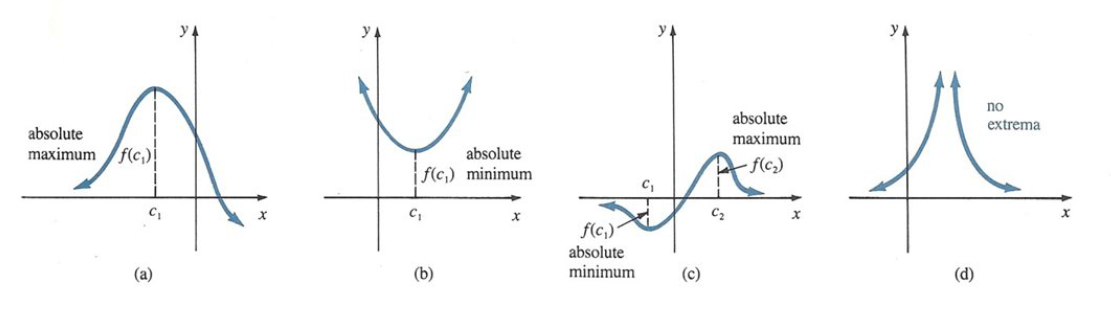
\includegraphics[width=0.8\textwidth]{good.png}\\[1cm]
  \end{center}
\noindent \textbf{Example:} The function $f(x)=x^2$ has the absolute minimum $f(0)=0$ but has no absolute maximum.

\noindent \textbf{Example:} $f(x)=\dfrac{1}{x}$ has neither an absolute maximum nor an absolute minimum.

\noindent The interval on which a function is defined is very important in the consideration of extrema. 

\noindent \textbf{Example:} $f(x)=x^2$ defined only on the closed interval $[1,2]$, has the absolute maximum $f(2)=4$ and the absolute minimum $f(1)=1$. On the other hand, if $f(x)=x^2$ is defined on the open interval $(1,2)$, then $f$ has no absolute extrema. In this case, $f(1)$ and $f(2)$ are not defined.

\begin{theorem}[Extreme Value Theorem]
A function $f$ continuous on $[a,b]$ always has an absolute maximum and an absolute minimum on the interval.
\end{theorem}
\begin{definition}
\begin{itemize}
\item[(i)] A number $f(c_1)$ is a \textbf{relative maximum} of a function $f$ if $f(x)\leq f(c_1)$ for every $x$ in some open interval that contains $c_1$.
\item[(ii)] A number $f(c_1)$ is a \textbf{relative minimum} of a function $f$ if $f(x)\geq f(c_1)$ for every $x$ in some open interval that contains $c_1$.
\end{itemize}
\end{definition}

\begin{definition}
A \textbf{critical value} of a function $f$ is a number $c$ in its domain for which $f'(c)=0$ or $f'(c)$ does not exist.
\end{definition}
\noindent \textbf{Example:} Find the critical values of $f(x)=x^3-15x+6$.

\noindent \textbf{Solution:} 
\begin{equation*}
f'(x)=3x^2-15.
\end{equation*}
The critical values are those numbers for which $f'(x)=0$, namely $\pm \sqrt{5}$.

\noindent \textbf{Example:} Find the critical value of $f(x)=(x+4)^{\frac{2}{3}}$.

\noindent \textbf{Solution:} By power rule for functions,  
\begin{equation*}
f'(x)=\dfrac{2}{3}(x+4)^{-\frac{1}{3}}=\dfrac{2}{3(x+4)^{\frac{1}{3}}}.
\end{equation*}
In this instance we see that $f'(x)$ does not exist when $x=-4$. Since $-4$ is in the domain of $f$, we conclude it is a critical value.

\begin{theorem}
If a function $f$ has a relative extremum at a number $c$, then $c$ is a critical value.
\end{theorem}
\section{Tutorial Questions}
\begin{enumerate}
\item Evaluate each of the following limits using L'hopital's rule.\\
(i)\, $\displaystyle \lim _{x\rightarrow 0}\dfrac{\sin x}{x}$ \quad (ii)\, $\displaystyle \lim _{x\rightarrow 0}\dfrac{\sin x}{e^x-e^{-x}}$ \quad (iii)\, $\displaystyle \lim _{x\rightarrow \infty}\dfrac{\ln x}{e^x}$ \quad (iv)\, $\displaystyle \lim _{x\rightarrow \infty}\dfrac{6x^2-5x+7}{4x^2-2x}$\\
(v)\, $\displaystyle \lim _{x\rightarrow \infty}\dfrac{e^{3x}}{x^2}$ \quad (vi)\, $\displaystyle \lim _{x\rightarrow \infty}\dfrac{x^4}{e^{2x}}$ \quad (vii)\, $\displaystyle \lim _{t\rightarrow {\frac{\pi}{4}}^+}\dfrac{\tan t}{\tan 3t}$ \quad (viii)\, $\displaystyle \lim _{x\rightarrow {1}^+}\dfrac{\ln x}{\sqrt{x-1}}$\\
(ix)\, $\displaystyle \lim _{x\rightarrow 0}\left[\dfrac{1+3x}{\sin x}-\dfrac{1}{x}\right]$ \quad (x)\, $\displaystyle \lim _{x\rightarrow \infty}x\sin \left(\frac{1}{x}\right)$ \quad (xi)\, $\displaystyle \lim _{x\rightarrow 0} x^{\frac{1}{\ln x}}$ \quad (xii)\, $\displaystyle \lim _{x\rightarrow 0}(1+x)^{\frac{1}{x}}$\\
(xiii)\, $\displaystyle \lim _{x\rightarrow \infty}\left(1-\frac{3}{x}\right)^{2x}$ \quad (xiv)\, $\displaystyle \lim _{x\rightarrow 0^+}x^x$ \quad (xv)\, $\displaystyle \lim _{x\rightarrow \infty}x(e^{\frac{1}{x}}-1)$ \quad (xvi)\, $\displaystyle \lim _{x\rightarrow 0}\left(\dfrac{1}{x}-\dfrac{1}{\sin x}\right)$.
\item Evaluate each of the following limits using L'Hopital's rule.\\
(i)\, $\displaystyle \lim _{x\rightarrow \infty}(2+e^x)^{e^{-x}}$ \quad (ii)\, $\displaystyle \lim _{x\rightarrow 0^-}(1-e^x)^{x^2}$ \quad (iii)\, $\displaystyle \lim _{x\rightarrow \infty}x^2e^{-x}$ \quad (iv)\, $\displaystyle \lim _{x\rightarrow \infty} (x+e^x)^{\frac{2}{x}}$\\
(v)\, $\displaystyle \lim _{x\rightarrow 0}x\ln (\sin x)$ \quad (vi)\, $\displaystyle \lim _{x\rightarrow 0}x^{\ln ^2 x}$ \quad (vii)\, $\displaystyle \lim _{x\rightarrow 0}(1+5\sin x)^{\cot x}$ \quad (viii)\, $\displaystyle \lim _{x\rightarrow \infty}\left(\dfrac{3x}{3x+1}\right)^x$\\
(ix)\, $\displaystyle \lim _{x\rightarrow 0}x^{(1-\cos x)}$ \quad (x)\, $\displaystyle \lim _{t\rightarrow \infty}\left(1+\frac{3}{t}\right)^t$ \quad (xi)\, $\displaystyle \lim _{x\rightarrow 0}\left(\dfrac{1}{e^x-1}-\dfrac{1}{x}\right)$ \quad (xii)\, $\displaystyle \lim _{x\rightarrow 0}\dfrac{\tan x}{2x}$\\
(xiii)\, $\displaystyle \lim _{x\rightarrow 0^+}(1+x)^{\frac{1}{x^2}}$ \quad (xiv)\, $\displaystyle \lim _{x\rightarrow {\frac{\pi}{2}}^+}(\sin ^2 x)^{\tan x}$ \quad (xv)\, $\displaystyle \lim _{\theta\rightarrow 0}\theta \csc 4\theta$ \quad (xvi)\, $\displaystyle \lim _{x\rightarrow 0^+}x\ln x$.
\item Evaluate each of the following using L'hopital's rule.\\
(i)\, $\displaystyle \lim _{r\rightarrow 0}\dfrac{r-\cos r}{r-\sin r}$ \quad (ii)\, $\displaystyle \lim _{x\rightarrow -\infty}\dfrac{1+e^{-2x}}{1-e^{-2x}}$ \quad (iii)\, $\displaystyle \lim _{x\rightarrow 0}\dfrac{e^x-x-1}{2x^2}$ \quad 
(iv)\, $\displaystyle \lim _{x\rightarrow 0}\dfrac{x-\tan ^{-1}x}{x-\sin ^{-1} x}$\\ (v)\, $\displaystyle \lim _{x\rightarrow 0^+}(\cos x)^{\frac{1}{x^2}}$ \quad (vi)\, $\displaystyle \lim _{x\rightarrow \infty}\left(1+\frac{a}{x}\right)^x$ \quad (vii)\, $\displaystyle \lim _{x\rightarrow \infty}x^{\frac{1}{x}}$ \quad (viii)\, $\displaystyle \lim _{x\rightarrow \frac{\pi}{4}}(\tan x)^{\tan x}$\\
(ix)\, $\displaystyle \lim _{x\rightarrow 0}(x^2)^x$ \quad (x)\, $\displaystyle \lim _{x\rightarrow 0}x^3\ln x$ \quad (xi)\, $\displaystyle \lim _{x\rightarrow 0}\dfrac{3^x-2^x}{x}$ \quad (xii)\, $\displaystyle \lim _{x\rightarrow 1^+}(\ln x)^{\ln x}$\\
(xiii)\, $\displaystyle \lim _{x\rightarrow 0}x^{\sin x}$ \quad (xiv)\, $\displaystyle \lim _{x\rightarrow \infty}(1+2x)^{\frac{1}{3x}}$ \quad (xv)\, $\displaystyle \lim _{x\rightarrow 0}\left(\dfrac{e^x\sec x}{x}-\dfrac{\sin x}{x^2}\right)$ \quad (xvi)\, $\displaystyle \lim _{x\rightarrow \infty}\dfrac{(x^2+3x+3)^{x+1}}{(x+1)^{2x+1}(x+2)}$.

\end{enumerate}
\section{Graphing and the First Derivative}
Knowing that a function does, or does not, possess relative extrema is a great aid in drawing its graph. 
\begin{theorem}
Let $f$ be continuous on $[a,b]$ and differentiable on $(a,b)$, except possibly at the critical value $c$.
\begin{itemize}
\item[(i)] If $f'(x)>0$ for $a<x<c$ and $f'(x)<0$ for $c<x<b$, then $f(c)$ is a \textbf{relative maximum}.
\item[(ii)]  If $f'(x)<0$ for $a<x<c$ and $f'(x)>0$ for $c<x<b$, then $f(c)$ is a \textbf{relative minimum}.
\item[(iii)] If $f'(x)$ has the same algebraic sign on $a<x<c$ and $c<x<b$, then $f(c)$ is not an extremum.
\end{itemize}
\end{theorem}
\begin{center}
 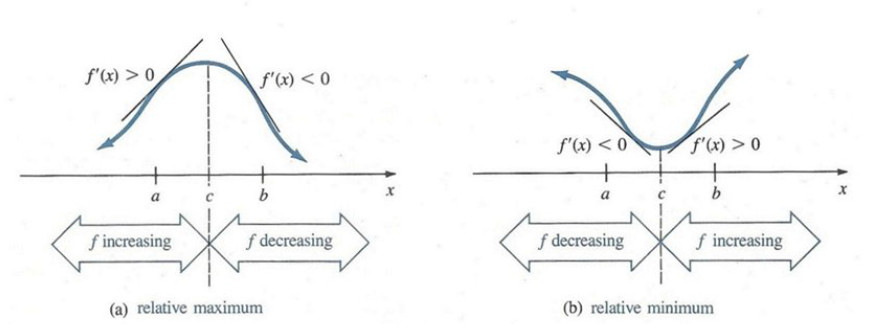
\includegraphics[width=0.8\textwidth]{min.png}\\[1cm]
  \end{center}
\noindent \textbf{Example:} For each of the following functions, find all the critical points and classify each as a relative maximum, relative minimum or neither. (a)\, $f(x)=3x^{\frac{5}{3}}-15x^{\frac{2}{3}}$ and (b)\, $f(x)=x^3-3x^2+3x-1$.

\noindent \textbf{Solution:} (a)\,\underline{Critical points:}
\begin{eqnarray*}
f'(x) &=& 5x^{\frac{2}{3}}-10x^{-\frac{1}{3}}\\
&=& 5x^{-\frac{1}{3}}(x-2)\\
&=& \dfrac{5(x-2)}{x^{\frac{1}{3}}},
\end{eqnarray*}
which is zero when $x=2$ and undefined when $x=0$. Therefore $x=0$ is a relative maximum and $x=2$ is a relative minimum.

\noindent (b)\, \underline{Critical points:}
\begin{eqnarray*}
f'(x) &=& 3x^2-6x+3 \\
&=& 3(x^2-2x+1)\\
&=& 3(x-1)^2, 
\end{eqnarray*}
which is defined everywhere and zero when $x=1$. Therefore $x=1$ is neither.

\noindent Sometimes there is an easier way to test a critical point. Our goal is to relate the concept of the concavity of a graph with the second derivative of a function. Often a shape that is concave upwards is said to ``hold water'' whereas a shape that is concave downwards ``spills water''.
\begin{definition}
Let $f$ be differentiable on $(a,b)$.
\begin{itemize}
\item[(i)] If $f'$ is an increasing function on $(a,b)$, then the graph of $f$ is \textbf{concave upwards} on the interval.
\item[(ii)]  If $f'$ is a decreasing function on $(a,b)$, then the graph of $f$ is \textbf{concave downwards} on the interval
\end{itemize}
\end{definition}
\begin{center}
 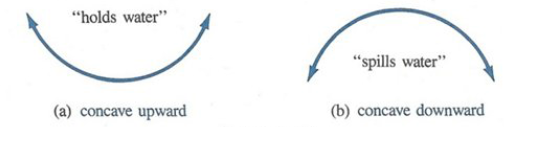
\includegraphics[width=0.5\textwidth]{great.png}\\[1cm]
  \end{center}
\begin{theorem}[Test for Concavity] Let $f$ be a function for which $f''$ exists on $(a,b)$.
\begin{itemize}
\item[(i)] If $f''(x)>0$ for all $x$ in $(a,b)$, then the graph is concave upward on $(a,b)$.
\item[(ii)] If $f''(x)<0$ for all $x$ in $(a,b)$, then the graph is concave downward on $(a,b)$.
\end{itemize}
\end{theorem}
\begin{center}
 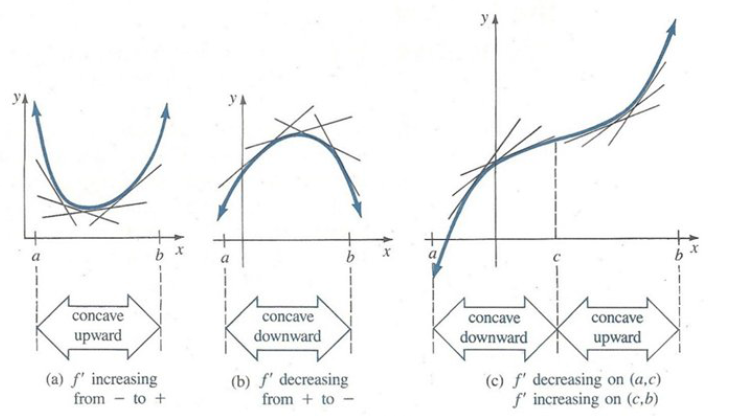
\includegraphics[width=0.6\textwidth]{turn.png}\\[1cm]
  \end{center}
\noindent \textbf{Example:} Determine the intervals on which the graph of $f(x)=-x^3+\frac{9}{2}x^2$ is concave upward and the intervals for which the graph is concave downward.

\noindent \textbf{Solution:} From 
\begin{eqnarray*}
f'(x) &=& -3x^2+9x\\
f''(x) &=& -6x+9 =6\left(-x+\frac{3}{2}\right),
\end{eqnarray*}
we see that $f''(x)>0$ when $6\left(-x+\frac{3}{2}\right)>0 $ or $x<\frac{3}{2}$ and that $f''(x)<0$ when $6\left(-x+\frac{3}{2}\right)<0$ or $x>\frac{3}{2}$. It follows that the graph of $f$ is concave upward on $(-\infty , \frac{3}{2})$ and concave downward on $(\frac{3}{2}, \infty)$.

\subsection{Point of Inflection}
\begin{definition}
Let $f$ be continuous at $c$. A point $(c, f(c))$ is a \textbf{point of inflection} if there exists  an open interval $(a,b)$ that contains $c$ such that the graph of $f$ is either 
\begin{itemize}
\item[(i)] concave upward on $(a,c)$ and concave downward on $(c,b)$ or 
\item[(ii)] concave downward on $(a,c)$ and concave upward on $(c,b)$.
\end{itemize}
\end{definition}
\noindent As a consequence, we observe that \textit{a point of inflection $(c,f(c))$ occurs at a number $c$ for which $f''(c)=0$ or $f''(c)$ does not exist}.

\noindent \textbf{Example:} Find any points of inflection of $f(x)=-x^3+x^2$.

\noindent \textbf{Solution:} The first and second derivatives of $f$ are, respectively, 
\begin{equation*}
f'(x)=-3x^2+2x \quad \hbox{and}~~ f''(x)=-6x+2.
\end{equation*}
Since $f''(x)=0$ at $\frac{1}{3}$, the point $(\frac{1}{3}, \frac{2}{27})$ is the only possible point of inflection. Now, 
\begin{eqnarray*}
f''(x) &=& 6\left(-x+\frac{1}{3}\right)>0\quad  \hbox{for}~~ x<\frac{1}{3}\\
f''(x) &=& 6\left(-x+\frac{1}{3}\right)<0\quad  \hbox{for}~~ x>\frac{1}{3}, 
\end{eqnarray*}
implies that the graph of $f$ is concave upward on $(-\infty , \frac{1}{3})$ and concave downward on $(\frac{1}{3}, \infty)$. Thus $(\frac{1}{3}, f(\frac{1}{3}))$ or $(\frac{1}{3}, \frac{2}{27})$ is a point of inflection.

\noindent \textbf{Second Derivative Test.} If $c$ is a critical value of $y=f(x)$ and, say, $f''(c)>0$, then the graph of $f$ is concave upward on some interval $(a,b)$ that contains $c$.  Necessarily then, $f(c)$ is a relative minimum. Similarly, $f''(c)<0$ at a critical value $c$ implies $f(c)$ is a relative maximum.
\begin{theorem}[Second Derivative Test for Relative Extrema] Let $f$ be a function for which $f''$ exists on an interval $(a,b)$ that contains the critical number $c$. 
\begin{itemize}
\item[(i)] If $f''(c)>0$, then $f(c)$ is a relative minimum.
\item[(ii)] If $f''(c)<0$, then $f(c)$ is a relative maximum.
\end{itemize} 
\end{theorem}
\begin{center}
 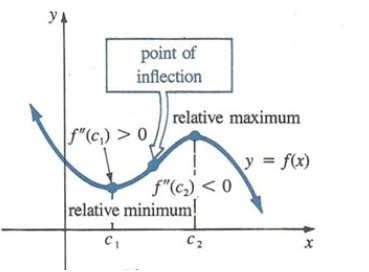
\includegraphics[width=0.3\textwidth]{point.png}\\[1cm]
  \end{center}
\noindent However, if $f''(c)=0$ then nothing can be concluded about the nature of the critical point.

\noindent \textbf{Example:} for each of the following functions, find all of the critical points and classify each as relative maximum, relative minimum or neither. (a)\, $f(x)=x^3-3x+2$ \quad (b)\, $f(x)=\frac{1}{2}x-\sin x$ on $0<x<2\pi$.

\noindent \textbf{Solution:} (a)\, 
\begin{eqnarray*}
f'(x) &=& 3x^2-3 \\
&=& 3(x^2-1) =3(x-1)(x+1),
\end{eqnarray*}
which is defined everywhere and zero at $x=1$ and $x=-1$. Computing $f''(x)=6x$, then 
\begin{eqnarray*}
f''(-1) &=& -6<0 \Rightarrow \hbox{relative maximum at}~~x=-1.\\
f''(1) &=& 6>0 \Rightarrow \hbox{relative minimum at}~~ x=1.
\end{eqnarray*}

\noindent (b)\, $f'(x)=\frac{1}{2}-\cos x$ which is defined everywhere and zero when $\cos x =\frac{1}{2}\Rightarrow x=\frac{\pi}{3}, \frac{5\pi}{3}$. Computing $f''(x)=\sin x$, then 
\begin{eqnarray*}
f''\left(\frac{\pi}{3}\right) &=& \sin \frac{\pi}{3} =\frac{\sqrt{3}}{2} >0 \Rightarrow \hbox{relative minimum at}~~x=\frac{\pi}{3}.\\
f''\left(\frac{5\pi}{3}\right) &=& \sin \frac{5\pi}{3} =-\frac{\sqrt{3}}{2} <0 \Rightarrow \hbox{relative maximum at}~~x= \frac{5\pi}{3}.
\end{eqnarray*}

\section{Sketching the graph of $y=f(x)$}
\section{Tutorial Questions}
\begin{enumerate}
\item Use differentials to compute approximate value of \\
(i)\, $\sqrt[3]{25}$ \quad (ii)\, $\sin 31^\circ$ \quad (iii)\, $\ln (1.12)$ \quad (iv)\, $\sqrt[5]{36}$ \quad (v)\, $\sqrt[5]{31}$ \quad (vi)\, $\cos 62^\circ$ \\
 (vii)\, $\sin 48^\circ$ \quad (viii)\, $(1005)^{\frac{1}{3}}$ \quad (ix)\, $\tan 31^\circ$ \quad (x)\, $\ln (1.2)$ \quad (xi)\, $\sqrt{26}$ \quad (xii)\, $\tan ^{-1}(1.1)$ \\ (xiii)\, $(1.1)^2+6(1.1)^2$ \quad (xiv)\, $\sin 1^\circ$ \quad (xv)\, $\dfrac{1}{\sqrt{96}}$.
 \item Verify Rolle's Theorem for $f(x)=x^2(1-x)^2, \quad 0\leq x\leq 1$.
 \item Find the value of $c$ in Rolle's Theorem when $f(x)=(x-a)^m(x-b)^n$ where $m$ and $n$ are positive integers.
 \item If $f'(x)\leq 0$ at all points of $(a,b)$, prove that $f(x)$ is monotonic decreasing in $(a,b)$. Under what conditions is $f(x)$ strictly decreasing in $(a,b)$?
 \item Use the mean value theorem to show that $\sin x \leq x$ and $\tan x\geq x$. Hence show that $\dfrac{\sin x}{x}$ is strictly decreasing on $(0,\frac{\pi}{2})$.
 \item Suppose $f$ and $g$ are continuous on $[a,b]$, differentiable on $(a,b)$ and $f'(x)=g'(x)$ for all $x\in (a,b)$. Show that $f(x)=g(x)+c$, where $c$ is a constant.
 \item Use the mean value theorem, to prove that, if $0<a<b$, then $(1-\frac{a}{b})<\ln(\frac{b}{a})<(\frac{b}{a}-1)$. Hence show that $\frac{1}{6}<\ln (1.2)<\frac{1}{5}$.
 \item Show that if $0<a<b$, then $\dfrac{b-a}{\sqrt{1-a^2}}<\sin ^{-1} (b)-\sin ^{-1}(a)<\dfrac{b-a}{\sqrt{1-b^2}}$. Hence show that $\left(\dfrac{\pi}{6}+\dfrac{\sqrt{3}}{15}\right)<\sin ^{-1}(0.6)<\left(\dfrac{\pi}{6}+\dfrac{1}{8}\right)$.
 \item Use the Mean Value Theorem to prove the following inequalities
 \begin{itemize}
 \item[(i)] $\ln (1+x) < x$ if $x>0$.
 \item[(ii)] $\sqrt{1+x} <1+\frac{1}{2}x$ if $x>0$.
 \item[(iii)] $\dfrac{x-1}{x}<\ln x <x-1$ for $x>1$.
 \end{itemize}
\item Find the relative extrema of the given functions.\\
(i)\, $f(x)=2x^3+3x^2-36x$ \quad (ii)\, $f(x)=x^5-\frac{5}{3}x^3+2$ \quad (iii)\, $4x-6x^{\frac{2}{3}}+2$ \\ (iv)\, $f(x)=\dfrac{x^2-2x+2}{x-1}$.
\item Find the relative extrema and the points of inflection of the following functions.\\
(i)\, $f(x)=x^4+8x^3+18x^2$ \quad (ii)\, $f(x)=x^6-3x^4+5$ \quad (iii)\, $f(x)=10-(x-3)^{\frac{1}{3}}$ \\
(iv)\, $f(x)=x(x-1)^{\frac{5}{2}}$.
\item Sketch the graphs of the following functions.\\
(i)\, $f(x)=2x^2-5x-3$ \quad (ii)\, $f(x)=\dfrac{x+1}{(x-2)(3x+5)}$ \quad (iii)\, $f(x)=x^4$ \quad (iv)\, $f(x)=x^9$\\
(v)\, $f(x)=\dfrac{2x-1}{(x+2)(x-3)}$ \quad (vi)\, $f(x)=\dfrac{x+1}{x-1}$ \quad (vii)\, $f(x)=\left(\dfrac{x+1}{x-1}\right)^2$.
\end{enumerate}
\end{document}